\subsection{Product perspective}
\subsubsection{Scenarios}
\begin{enumerate}[label=\textbf{\arabic*}.]
    \item \textbf{ Educator creates a tournament}\\Alan is a university professor. He has just finished explaining a very hard topic that occupied multiple lectures. He would like to test its class about it but exams dates are far away ahead and he thinks that trying to evaluate their understanding with a quick quiz performed in class before or after his next lecture would not be a good idea given the depth of the topic. Anyway he knows of a site that allows educators to easily organize challenges to which students can take part and decides to give it a try.\\He connects to the website of the platform and signs up as an educator. After that, he navigates to the “Tournaments” section and selects the option to create a new one: inputs the name of the tournament and a deadline for the subscription. All students subscribed to the CKB platform are now notified and can join the tournament.\\Since Alan’s schedule is often very busy, he then decides to grant the permission to create battles to his teaching assistant Thomas, which has already subscribed to the platform.
    \item \textbf{ Educator creates a battle}\\Linus is a famous youtuber that publishes video courses on programming languages. He wants to increase the engagement with his subscribers, so for this reason he has already subscribed to the CKB platform and created a tournament. In his last video lecture, he has started a new playlist on Java language, explaining some basic concepts typical of object oriented programming.\\To challenge his viewers, he decides to create a new coding battle. He now connects to the website of the platform and log-ins with his credential. He clicks on the tournament called “LinusTechChallenges” he previously created and selects the option to generate a new battle. The platform then asks him to specify some settings for this specific challenge: he selects “Java” as programming language, uploads the “code kata” which includes a textual description of the challenge and all the files related to the software project like test cases and build automation scripts, selects set the minimum and maximum number of students per group, fixes the registration and final submission deadlines. Since he has many subscribers and cannot manually review every solution, he also specifies that a final manual evaluation is not needed. However, Linus decides to enable all the available aspects the static analysis should focus on (e.g. security, reliability, maintainability). At this point he confirms the creation of the battle and the system automatically notifies all the students subscribed to the tournament about the new coding battle.
    \item \textbf{ Student subscribes to a tournament}\\Mark is struggling to keep the pace of its professor’s lectures. Moreover, since his anxiety always penalizes him, he is afraid he will organize some activity in class to evaluate his knowledge about the last, complex topic. One day, while looking at the academic mail, he notices that the feared professor is contacting its students to inform them of an alternative evaluation method that would allow them to avoid part of the final exam and which involves to write code to solve problems related with the subject and compete with other students. Mark immediately decides to go for it and subscribes (as a student) to the platform indicated by the professor. Once logged in, he goes to the “Tournaments” section and selects the option to search for a specific tournament: at this point he searches the tournament by the name communicated by the professor, selects it and subscribes to it. Once a new battle will be available, he will be notified by the system. He is now ready to participate to the battles and prove what he has learned.
    \item \textbf{ Students form a team}\\Liam is a software engineer that has subscribed to CKB because a famous IT company is offering some job positions to the most talented developers discovered through the platform. For this reason, he already joined the tournament created by the company. Since the company is interested in developers with the ability to work in teams, its human resources department has set “2” as minimum number of team members for their first battle. So, Liam decides to tackle the first challenge with a trusted former university colleague of his. He navigates to the “Tournaments” section, searches and selects the ongoing tournament of the company and clicks on the first battle called “Challenge 1”. The system shows 2 options: “Create a team” and “Join a team”. Liam selects the first option and chooses a name for his team, checking the “private” flag option. The systems generates an invite code that he can now share privately to his friend in order to join the team.
    \item \textbf{ Student submits a solution}\\Jonas is subscribed to the CKB platform in order to participate in quizzes organized by his computer science professor. He is very happy with this kind of continual evaluation because it's a great way to understand those difficult concepts taught during theory classes and skip some exercises at the final written exam.\\When a new programming challenge is announced, Jonas gets excited to test his skills. He forms a team with two other classmates to collaborate on solving the exercise. After working hard to come up with a new solution, Jonas submits it to the CKB platform by committing the solution on their GitHub repository before the deadline. Jonas and his team mates have monitored their score during the whole battle, but are not satisfied with rank of their final submission computed with the automated evaluation.\\The next day, after the consolidation stage, Jonas is thrilled to see his final team rank near the top of the leaderboard! Indeed the professor liked a lot their innovative solution and decided to  reward them during the manual evaluation.
    \item \textbf{ Educator manually evaluates solutions}\\Oliver is an instructor and he is using CKB to evaluate the students enrolled in his online programming course. He enjoys the platform because it organizes the students’ GitHub repository in a convenient and central way. Indeed, once the submission phase ends, during the consolidation stage Oliver can select the current battle and go through the whole list of teams. For each team, the system shows the GitHub repository link and the scores related to the automated evaluation. After inspecting the code in the repo, Oliver inputs in the same page a natural number between 0 and 100 as manual evaluation score (the higher the better). Once he has finished reviewing the code of all the teams, he clicks on the “Terminate battle” field next to the current battle tab and all students involved are notified about the final mark.
\end{enumerate}

\subsubsection{Domain Class diagram}
\begin{figure}[H]
    \hspace{-98px}
    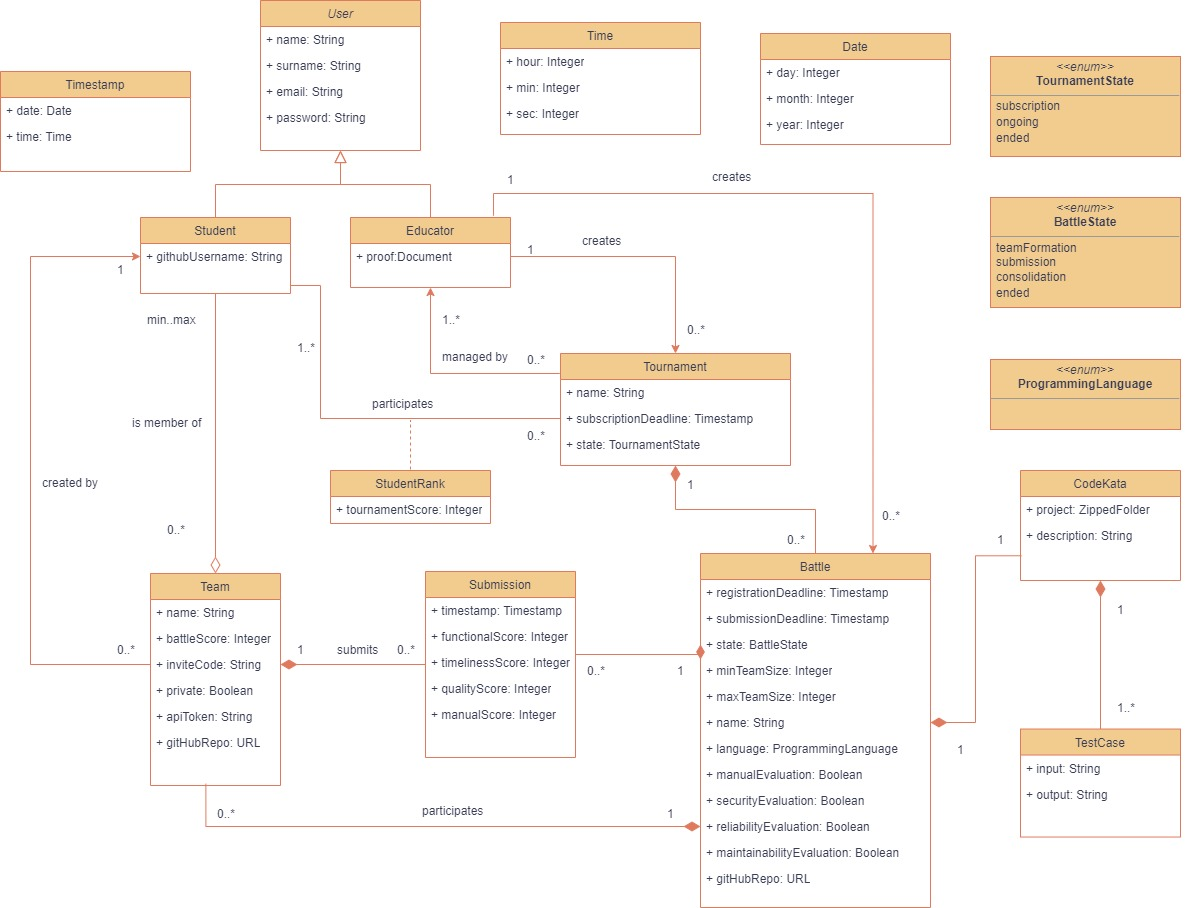
\includegraphics[scale=0.5]{Diagrams/uml_v2.jpg}
    \caption{Domain-level UML diagram}
    \label{class_diagram}
\end{figure}
\newpage
\textbf{ Additional notes on the class diagram:}
\begin{itemize}
    \item the “created by” relation between "Student" and "Team" encapsulates the concept of "team leader".
    \item the "proofDocument" attribute of the "Educator" class contains a reference to the file through which the educator was verified.
\end{itemize}

\subsubsection{ State diagrams}
In order to provide a complete description of the application domain, here we included the state diagrams relative to battles and tournaments.
\begin{figure}[h]
    \centering
    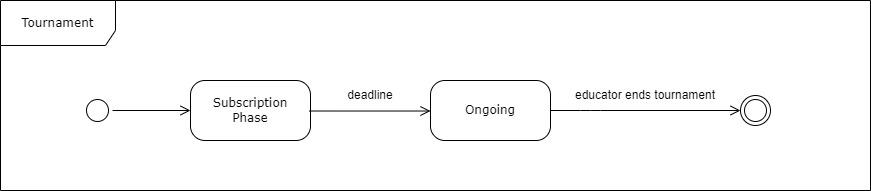
\includegraphics[scale=0.4]{Diagrams/tournament_state.jpg}
    \caption{Tournament state diagram}
    \label{tournament_state}
\end{figure}
\begin{figure}[h]
    \centering
    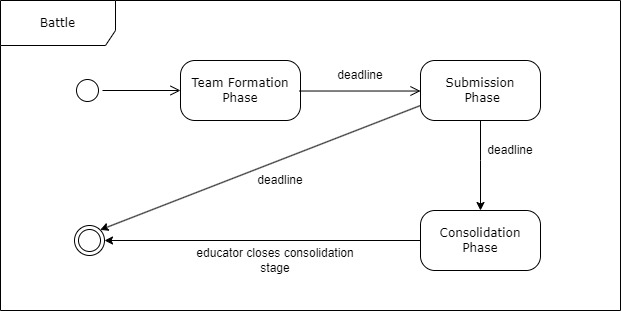
\includegraphics[scale=0.4]{Diagrams/battle_state.jpg}
    \caption{Battle state diagram}
    \label{battle_state}
\end{figure}
\\In particular, in the case of battles, which transition is taken after the submission stage only depends on whether the manual evaluation was enabled or not.